% !TeX program=pdflatex
\documentclass{standalone}
\usepackage{blindtext}
\usepackage{pgfplots}
\pgfplotsset{compat=1.9}

\begin{document}
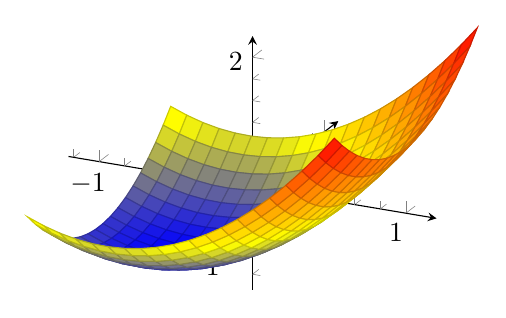
\begin{tikzpicture}[
        declare function = {
            q(\x) = \x - 1;
  %          R(\x,\y)=sqrt(\x^2+\y^2);
 %           Phi(\x,\y)=acos(\x/\y)
            Z(\x,\y) = \x^2 + \y^2 + q(\x);
%           Z(\x,\y) = \Zinit+sin(R(\x,\y)/\RMax*\pi/2)^2*(\A-\B*cos(3*Phi(\x,\y)))";
        }
    ]
    \begin{axis}
    [
    axis lines=center,
    enlargelimits,
    tick align=inside,
    domain=-1:1,
    samples=20, % this was 200, but I changed it to 20 because of my slow PC
    minor tick num=5,
    ]
    \addplot3 [surf] {Z(x,y)};
    \end{axis}
\end{tikzpicture}
\end{document}